\chapter{Variáveis Aleatórias e Suas Distribuições}

\section{Variáveis Aleatórias}
 
Uma variável aleatória é uma quantidade de interesse cujo valor verdadeiro é desconhecido. Para obter informações sobre uma variável aleatória, é necessário projetar e conduzir experimentos. É inerente a qualquer experimento que a variável aleatória de interesse nunca será conhecida exatamente. Em vez disso, a variável será caracterizada por uma \textbf{função de distribuição de probabilidade}, que determina qual é a probabilidade de que um determinado valor da variável aleatória ocorra. Repetir a medição geralmente aumenta o conhecimento da distribuição da variável: essa é a razão para querer medir a quantidade o máximo possível.

Exemplos de variáveis aleatórias são a massa da Terra, a altura da Torre Eiffel ou a voltagem de uma tomada elétrica. A natureza aleatória de praticamente todas as quantidades reside principalmente no fato de que nenhuma quantidade é conhecida exatamente por nós sem realizar um experimento, e que nenhum experimento é perfeito devido a limitações práticas ou até teóricas. Entre as razões práticas estão, por exemplo, limitações na precisão do aparelho de medição. As razões teóricas dependem da natureza da variável. Por exemplo, a medição da posição e velocidade de uma partícula subatômica é limitada pelo princípio da incerteza de Heisenberg \citep{heisenberg1927anschaulichen}, que proíbe um conhecimento exato de ambas as quantidades mesmo na presença de um aparelho de medição perfeito.

O método geral para obter informações sobre uma variável aleatória $X$ começa com um conjunto de medições $x_i$, garantindo que as medições sejam realizadas sob as mesmas condições experimentais. A partir dessas medições, obtém-se uma distribuição da frequência de ocorrência de todos os valores de $X$ conhecida como a \textbf{distribuição amostral da variável}, que descreve a distribuição empírica dos valores coletados no experimento (\autoref{fig:2-1}). Espera-se também que uma variável aleatória tenha uma distribuição teórica, por exemplo, Gaussiana, uniforme, etc., de acordo com a natureza da própria variável e o método de medição. Esta distribuição teórica é referida como \textbf{distribuição populacional} e representa a crença de que existe uma descrição ideal da variável aleatória. Como será mostrado nos capítulos seguintes, espera-se que a distribuição amostral se torne a distribuição populacional se um número infinito de medições for realizado, de tal forma que a aleatoriedade associada a um pequeno número de medições seja eliminada.

\begin{SCfigure}[\sidecaptionrelwidth][ht!]
	\centering
	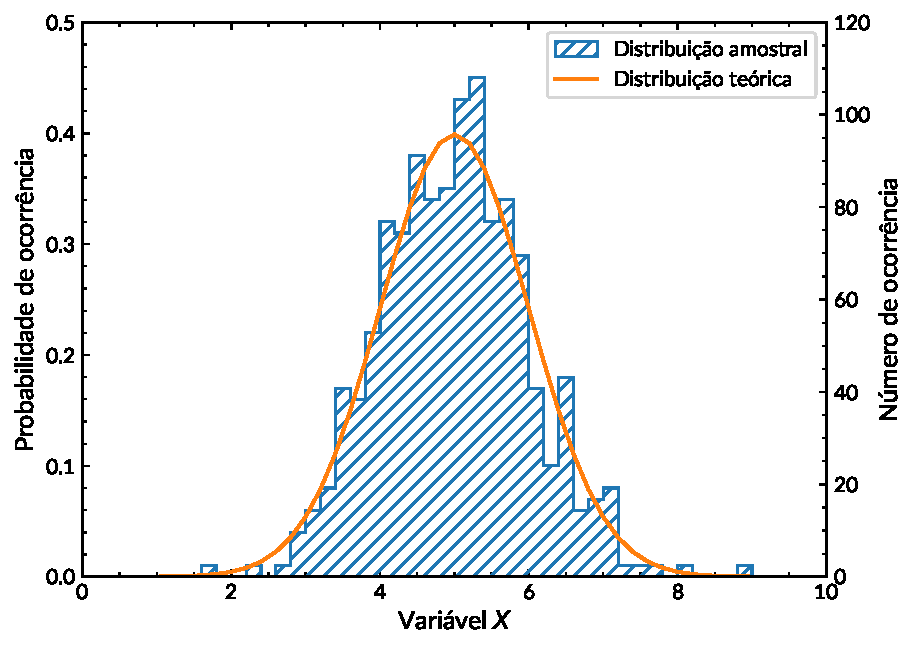
\includegraphics[width=0.7\linewidth]{Figuras/2-1.pdf}
	\caption{Distribuição amostral de uma variável aleatória $X$ a partir de 500 medições, obtida combinando as medições em intervalos de largura igual ($\Delta x = 0.2$). A forma da distribuição teórica depende da natureza do experimento e do número de medições, e neste exemplo é representada pela curva laranja.}
	\label{fig:2-1}
\end{SCfigure}

\section{Funções de Distribuição de Probabilidade}

É conveniente definir uma função que descreve a probabilidade de ocorrência da variável aleatória. Variáveis aleatórias discretas são descritas por uma \textbf{função de massa de probabilidade} (FMP) $f(x_i)$, onde $f(x_i)$ representa a probabilidade da variável ter um valor exato de $x_i$. Variáveis contínuas são descritas por uma \textbf{função de densidade de probabilidade} (FDP) $f(x)$, de modo que $f(x)\,dx$ é a probabilidade da variável estar no intervalo $[x, x + dx]$. Para simplicidade, a maioria das propriedades será ilustrada para variáveis contínuas, com a compreensão de que elas também se aplicam a variáveis discretas com modificações simples, como a substituição de uma integral por uma soma. Em princípio, também é possível ter variáveis aleatórias mais complexas que são parcialmente contínuas e parcialmente discretas. Um tratamento mais completo das variáveis aleatórias pode ser encontrado em qualquer livro-texto dedicado ao assunto, como os de \citet{ross2019introduction} ou \citet{siegrist2019random}. As funções de distribuição de probabilidade têm as seguintes propriedades-chave:

\begin{enumerate}[noitemsep]
\item Elas são normalizadas para 1. Para variáveis contínuas, isso significa que 
\begin{equation}
\int_{-\infty}^{\infty} f(x)\,dx = 1.
\end{equation}
Para variáveis definidas em um subconjunto dos números reais, por exemplo, apenas valores $x \geq 0$ ou em um intervalo finito, $f(x)$ é definido como zero fora do domínio de definição da função. Para variáveis discretas, a integral é substituída por uma soma sobre todos os valores que a variável pode assumir.

\item A distribuição de probabilidade nunca pode ser negativa, $f(x) \geq 0$. Isso é uma consequência do axioma de Kolmogorov, que requer que a probabilidade seja não negativa.

\item A \textbf{função de distribuição acumulada} (FDA) $F(x)$, ou simplesmente \textbf{função de distribuição}, 
\begin{equation}
F(x) = P(X \leq x) = \int_{-\infty}^{x} f(\tau)\, d\tau,
\end{equation}
representa a probabilidade de que a variável tenha um valor menor ou igual a $x$. $F(x)$ é uma função não decrescente de $x$ que começa em zero e tem seu maior valor de um. Uma função relacionada é a \textbf{função de sobrevivência} $S(x) = 1 - F(x)$, representando a probabilidade de $X > x$.
\end{enumerate}

\begin{exemplo}{}{}
A variável aleatória exponencial segue a FDP:
\begin{equation}
f(x) = \lambda e^{-\lambda x}, \quad x \geq 0,
\end{equation}
onde $\lambda$ é um parâmetro que deve ser positivo. Portanto, a FDP é $f(x) = 0$ para valores negativos da variável. A FDA é dada por:
\begin{equation}
F(x) = \int_{-\infty}^{x} \lambda e^{-\lambda \tau}\, d\tau =  \int_{-\infty}^{0} \lambda e^{-\lambda \tau}\, d\tau + \int_{0}^{x} \lambda e^{-\lambda \tau}\, d\tau  = 0 + \lambda\left(-\dfrac{1}{\lambda}e^{-\lambda \tau}\right)_0^{x} = 1 - e^{-\lambda x}.
\end{equation} 
Na \autoref{fig:2-2} estão representadas a FDP $f(x)$ e a FDA $F(x)$ para uma variável exponencial com $\lambda = 0.5$.
\begin{center}
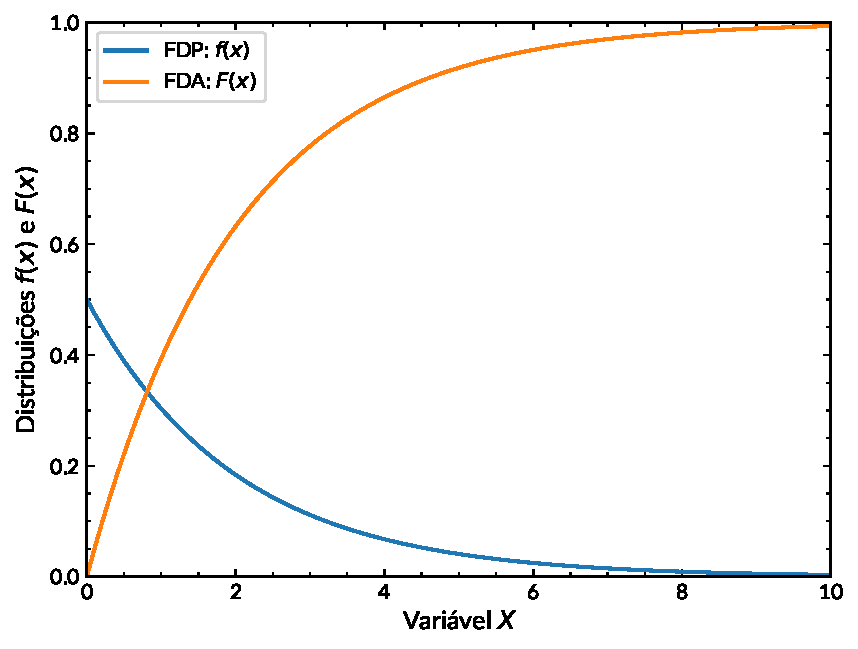
\includegraphics[width=0.65\linewidth]{Figuras/2-2.pdf}
\captionof{figure}{A função de distribuição $f(x)$ e a função de distribuição acumulada $F(x)$ para uma variável exponencial com $\lambda = 0.5$.}
\label{fig:2-2}
\end{center}
\end{exemplo}

\section{Expectância e Momentos de uma Função de Distribuição}

A função de densidade de probabilidade $f(x)$ ou a função de distribuição $F(x)$ fornece uma descrição completa da variável aleatória $X$. É conveniente encontrar algumas quantidades que descrevem os recursos mais importantes da distribuição. A \textbf{expectância} (ou \textbf{valor esperado}) de uma função determinística $g(x)$ da variável aleatória é definida por
\begin{equation}
\mathbb{E}[g(X)] = \int g(x) f(x)\, dx.
\end{equation}
O significado dessa expressão é que cada valor $g(x)$ é ponderado de acordo com a probabilidade de ocorrência de $x$, que é $f(x)$. A expectância é um operador linear, ou seja, satisfaz a propriedade
\begin{equation*}
\mathbb{E}[ag_1(x) + bg_2(x)] = a\,\mathbb{E}[g_1(x)] + b\,\mathbb{E}[g_2(x)]
\end{equation*}
devido à propriedade de linearidade da integral.

O \textbf{momento} de ordem $n$ é definido como
\begin{equation}
\mu_n = \mathbb{E}[X^n] =  \int x^n f(x)\, dx.
\end{equation}
Portanto, o momento $\mu_n$ é a expectância da função $g(x) = x^n$. É possível demonstrar, embora além do escopo deste livro, que o conhecimento dos momentos de todas as ordens é suficiente para determinar unicamente a função de distribuição \citep{wilks1947mathematical}. Este é um fato importante, pois transfere o problema de determinar a função de distribuição para o de determinar pelo menos alguns de seus momentos. Além disso, várias funções de distribuição têm apenas alguns momentos diferentes de zero, o que torna a tarefa ainda mais gerenciável.

Os momentos de uma distribuição são quantidades teóricas que podem ser calculadas a partir de  $f(x)$, sem qualquer referência a medidas. A seguir, são descritos dois dos momentos mais comumente utilizados, a média e a variância, e as quantidades amostrais que os aproximam, a média amostral e a variância amostral.

\subsection{A Média e a Média Amostral}

O momento de primeira ordem também é conhecido como \textbf{média} ou expectância da variável aleatória,
\begin{equation}\label{2.7}
	\mu = \mathbb{E}[X] = \int_{-\infty}^{\infty} x f(x)\, dx.
\end{equation}
A média $\mu$ é um número característico que representa um valor médio de $X$, obtido ponderando todos os valores possíveis da variável por sua função de distribuição. Portanto, a média é uma medida muito simples e conveniente da variável aleatória.

Para estimar a média da variável aleatória $X$, considere $N$ medidas $x_i$, com $i = 1, \ldots, N$. Cada medida $x_i$ pode ser considerada como uma amostra retirada aleatoriamente da distribuição populacional de $X$. A \textbf{média amostral} é definida como
\begin{equation}\label{2.8}
\overline{x} = \dfrac{1}{N} \sum_{i=1}^{N} x_i.
\end{equation}
É evidente que diferentes amostras de tamanho $N$ não resultarão no mesmo valor de $\overline{x}$, devido à aleatoriedade das medidas. Isso indica que $\overline{x}$ não é um número fixo, mas é ele próprio uma variável aleatória que deve ser escrita como
\begin{equation*}
	\overline{X} = \dfrac{1}{N} \sum_{i=1}^{N} X_i.
\end{equation*}
Esta nova equação é formalmente idêntica à \eqref{2.8} exceto pelo uso de letras maiúsculas, indicando que as quantidades são variáveis aleatórias, não apenas números. Portanto, é razoável perguntar se essa nova variável aleatória $\overline{X}$ tem a mesma expectância que a variável populacional $X$ em si. Essa pergunta pode ser facilmente respondida considerando que as variáveis $X_i$ são distribuídas de maneira idêntica da mesma forma que $X$, já que representam medidas aleatórias de $X$. A expectância de $\overline{X}$ é então:
\begin{equation*}
\mathbb{E}[\overline{X}] = \mathbb{E}\left[\dfrac{1}{N} \sum_{i=1}^{N} X_i\right] = \dfrac{1}{N}\sum_{i=1}^{N}\mathbb{E}[X_i] = \dfrac{N\mu}{N} = \mu.
\end{equation*}
A média amostral tem a mesma expectância que a variável populacional $X$, e portanto $\overline{X}$ é considerado um \textbf{estimador não tendencioso} de $X$. Esta é uma propriedade muito desejável, dado que a média amostral foi projetada exatamente com o propósito de estimar a variável populacional $X$ com suas medidas. Também se espera que, à medida que o número de medidas $N$ aumenta, a média amostral se aproxime cada vez mais da média populacional com maior precisão. Isso é mostrado na seção seguinte.

\subsection{A Lei dos Grandes Números}

A \textbf{lei dos grandes números} afirma que a média amostral converge para a média populacional conforme o tamanho da amostra aumenta, e é um dos teoremas fundamentais da probabilidade. Considere $N$ variáveis aleatórias $X_i$ que são identicamente distribuídas com $\mu$ sendo a média comum delas. A lei pode ser enunciada como:
\begin{equation}\label{2.9}
\lim\limits_{N \to \infty} \dfrac{X_1 + \cdots + X_N}{N} = \mu,
\end{equation}
Isso implica que a média amostral $X$ tende para a média $\mu$, que é um número determinístico e não uma variável aleatória. A \autoref{2.9} é uma afirmação muito forte porque mostra que, assintoticamente, a soma das variáveis aleatórias se torna uma constante igual à média amostral das $N$ variáveis, ou $N$ medidas. Embora não haja indicação sobre quão grande $N$ deve ser para alcançar esse objetivo, isso ainda é um resultado-chave para estabelecer o comportamento assintótico das variáveis aleatórias. É útil apontar que existem diferentes versões desta lei, de acordo com o método pelo qual essa convergência é estabelecida. Propriedades matemáticas desta lei e sua derivação podem ser encontradas em livros de teoria da probabilidade, como \citet{kolmogorov1950foundations,ross2019introduction}.

Essa lei também tem consequências importantes para funções de variáveis aleatórias. Dada uma função $g(x)$, seria conveniente estimar seu valor esperado $\mathbb{E}[g(X)]$ a partir das $N$ medidas das variáveis $X_i$. De acordo com a lei dos grandes números, é possível dizer que
\begin{equation}
	\lim\limits_{N \to \infty} \dfrac{g(X_1) + \cdots + g(X_N)}{N} = \mathbb{E}[g(X)].
\end{equation}
Essa expressão afirma que um grande número de medidas das variáveis $X_i$ pode ser usado para medir $\mathbb{E}[g(X)]$, contornando completamente a função de densidade de probabilidade da função $g(X)$. Essa propriedade será útil ao estudar a distribuição de funções de uma variável aleatória.

\subsection{A Variância e a Variância Amostral}

A \textbf{variância} é a expectância do quadrado da diferença entre $X$ e sua média,
\begin{equation}\label{2.11}
\text{Var}(X) = \mathbb{E}[(X - \mu)^2] = \int_{-\infty}^{+\infty} (x - \mu)^2 f(x)\,dx
\end{equation}
e geralmente é indicada como $\text{Var}(X) = \sigma^2$. A raiz quadrada da variância é referida como o \textbf{desvio padrão} $\sigma$, e é uma medida comum da diferença média de uma determinada medida $x_i$ da média da variável aleatória.

A principal razão para definir a média da diferença de uma medida de sua média em termos de um momento de segunda ordem é que a expectância da diferença $X - \mu$ é sempre zero:
\begin{equation*}
\mathbb{E}[X - \mu] = \mathbb{E}[X] - \mathbb{E}[\mu] = \mu - \mu = 0
\end{equation*}
Portanto, a diferença de uma variável aleatória não é comumente utilizada em estatísticas, uma vez que sua expectância é nula. Observe que as dimensões físicas dos momentos da ordem $n$ são aquelas da variável elevada à potência $n$. Por exemplo, se $X$ for medida em metros, a variância é medida em metros quadrados ($\text{m}^2$), enquanto o desvio padrão tem as mesmas dimensões que a variável e sua média.

Usando a propriedade linear da expectância, é simples mostrar que a seguinte propriedade se aplica:
\begin{equation}\label{2.12}
\text{Var}(X) = \mathbb{E}[(X - \mu)^2] = \mathbb{E}[X^2 - 2X\mu + \mu^2] = \mathbb{E}[X^2] - 2\mu^2 + \mu^2 = \mathbb{E}[X^2] - \mu^2.
\end{equation}
Essa relação é muito conveniente para calcular a variância a partir dos momentos de primeira e segunda ordem. Outra propriedade útil da variância, que decorre do fato de que a variância é um momento de segunda ordem, é
\begin{equation}\label{2.13}
\text{Var}(aX) = a^2 \cdot \text{Var}(X),
\end{equation}
onde $a$ é uma constante. O desvio e a variância são momentos calculados em relação à média, e são referidos como \textbf{momentos centrais}.

A \textbf{variância amostral} é definida como
\begin{equation}\label{2.14}
s^2 = \dfrac{1}{N -1} \sum_{i=1}^N (x_i - \overline{x})^2,
\end{equation}
uma nova variável aleatória que se destina a estimar a variância populacional $\sigma^2$ por meio de $N$ medições aleatórias. O fator $N - 1$, e não $N$, no denominador é necessário para garantir que a variância da amostra seja um estimador não tendencioso da variância populacional. Uma prova dessa propriedade é fornecida na \autoref{sec:2-6}.

\section{Covariância e Correlação entre Variáveis Aleatórias}

É comum medir mais de uma variável aleatória em um experimento dado. As variáveis frequentemente estão relacionadas entre si, e, portanto, é necessário definir uma medida de como uma variável afeta a medição das outras. Considere a medição tanto do comprimento de um lado de um quadrado quanto de sua área; é claro que as duas quantidades estão relacionadas de tal forma que a mudança de uma quantidade afeta a outra da mesma maneira, ou seja, uma mudança positiva no comprimento do lado resulta em uma mudança positiva na área. Nesse caso, o comprimento e a área serão ditos ter uma correlação positiva. Esta seção introduz conceitos-chave para estudar duas ou mais variáveis aleatórias simultaneamente.

\subsection{Distribuição de Probabilidade Conjunta e Momentos de Duas Variáveis Aleatórias}

Quando duas variáveis são medidas ao mesmo tempo, deseja-se saber a probabilidade de um par de medidas dado para as duas variáveis. Essa informação é fornecida pela \textbf{função de distribuição de probabilidade conjunta}, indicada como $h(x, y)$, onde $h(x, y)\,dxdy$ é a probabilidade de que as duas variáveis $X$ e $Y$ estejam em um intervalo bidimensional de tamanho $dxdy$ em torno do valor $(x, y)$. Essa função bidimensional pode ser representada experimentalmente por meio de sua distribuição amostral, da mesma forma que as distribuições unidimensionais.

Normalmente, é conveniente descrever o comportamento de uma variável de cada vez, mesmo que o experimento envolva mais de uma variável. O processo de considerar apenas uma variável de cada vez é chamado \textbf{marginalização}. A função de densidade de probabilidade marginal de $X$, ou seja, a função de distribuição de $X$ isoladamente, é obtida a partir da função de distribuição de probabilidade conjunta como:
\begin{equation}\label{2.15}
f_X(x) = \int_{-\infty}^{\infty} h(x,y) dy,
\end{equation}
com uma equação equivalente para a distribuição marginal de $Y$. A expectância de $X$ é definida como:
\begin{equation}
\mathbb{E}[X] = \int_{-\infty}^{\infty}\int_{-\infty}^{\infty} xh(x,y)\,dxdy = \mu_x,
\end{equation}
e similarmente a expectância de $Y$ é igual a:
\begin{equation*}
	\mathbb{E}[Y] = \int_{-\infty}^{\infty}\int_{-\infty}^{\infty} yh(x,y)\,dxdy = \mu_y.
\end{equation*}
A combinação dessas duas equações leva ao resultado:
\begin{equation*}
	\mathbb{E}[X + Y] = \int_{-\infty}^{\infty}\int_{-\infty}^{\infty} (x + y)h(x,y)\,dxdy = \mathbb{E}[X] + \mathbb{E}[Y],
\end{equation*}
o que significa que a expectância da soma de duas variáveis é igual à soma das expectâncias. Este é um resultado conveniente que se aplica a todas as variáveis aleatórias e pode ser generalizado para mais de duas variáveis, sendo geralmente referido como a propriedade linear da expectância. Em particular, é útil ressaltar que a propriedade linear se aplica independentemente da independência estatística entre as variáveis, que é introduzida mais adiante nesta seção.

A variância é definida de forma similar como:
\begin{equation}
\text{Var}(X) = \mathbb{E}[(X - \mu_x)^2] = \int_{-\infty}^{\infty}\int_{-\infty}^{\infty} (x - \mu_x)^2 h(x, y)\, dxdy = \sigma_x^2.
\end{equation}
Essas equações reconhecem o fato de que a outra variável, neste caso $Y$, é de fato parte do experimento, mas é considerada não interessante para o cálculo em questão. Portanto, a variável não interessante é integrada (ou somada) sobre, ponderada pela sua função de distribuição de probabilidade.

A \textbf{covariância} de duas variáveis aleatórias é definida como:
\begin{equation}\label{2.18}
\text{Cov}(X,Y) = \mathbb{E}[(X - \mu_x)(Y - \mu_y)] = \int_{-\infty}^{\infty}\int_{-\infty}^{\infty} (x - \mu_x)(y - \mu_y) h(x, y)\, dxdy
\end{equation}
e geralmente é representada como $\text{Cov}(X,Y) = \sigma_{xy}^2$. A covariância é a expectância do produto dos desvios das duas variáveis, e a ordem das duas variáveis é irrelevante, de modo que $\text{Cov}(X,Y) = \text{Cov}(Y,X)$. A covariância é positiva se, em média, um desvio positivo de $X$ for acompanhado por um desvio positivo de Y, ou se dois desvios negativos forem prováveis de ocorrer simultaneamente, de modo que o integrando seja uma quantidade positiva. Se, por outro lado, as duas variáveis tendem a ter desvios de sinais opostos, a covariância será negativa. A covariância, assim como a média e a variância, é uma quantidade populacional que pode ser calculada a partir da distribuição teórica das variáveis aleatórias. A covariância também pode ser calculada desenvolvendo o lado esquerdo da \autoref{2.18},
\begin{equation*}
	\text{Cov}(X,Y) = \mathbb{E}[(X - \mathbb{E}[X])(Y - \mathbb{E}[Y])] = \mathbb{E}[XY - X\mathbb{E}[Y] -\mathbb{E}[X]Y + \mathbb{E}[X]\mathbb{E}[Y]] = \mathbb{E}[XY] - \mathbb{E}[X]\mathbb{E}[Y],
\end{equation*}
e possui as seguintes propriedades lineares:
\begin{equation*}
\text{Cov}(X + a,Y + b) = \text{Cov}(X,Y) \qquad \text{e} \qquad \text{Cov}(aX + b,cY + d) = ac \cdot \text{Cov}(X,Y),
\end{equation*}
o que pode ser visto imediatamente a partir da definição de covariância e da propriedade linear da expectância. Outra propriedade útil é:
\begin{equation*}
	\text{Cov}(X + Z,Y) = \text{Cov}(X,Y) +\text{Cov}(Z,Y),
\end{equation*}
que pode ser comprovada expandindo as expectâncias, e pode ser generalizada para mais de duas variáveis.

A \textbf{covariância amostral} para uma coleção de $N$ pares de medidas é calculada como:
\begin{equation}\label{2.19}
	s_{xy}^2 = \dfrac{1}{N-1}\sum_{i=1}^N(x_i - \overline{x})(y_i - \overline{y}),
\end{equation}
usando uma equação similar à variância amostral. É possível mostrar que o denominador $(N - 1)$ é necessário para garantir que a covariância amostral seja um estimador não tendencioso da covariância populacional. Essa derivação é fornecida na \autoref{sec:2-6}.

A \textbf{correlação} é simplesmente uma versão normalizada da covariância:
\begin{equation}
\text{Cor}(X,Y) = \dfrac{\text{Cov}(X,Y)}{\sqrt{\text{Var}(X)\text{Var}(Y)}} = \dfrac{\sigma_{xy}^2}{\sigma_x\sigma_y},
\end{equation}
e pode ser indicada como $\text{Cor}(X,Y) = \rho$. A \textbf{desigualdade de Cauchy-Schwarz} é frequentemente declarada como:
\begin{equation}
\mathbb{E}[|XY|] \leq \sqrt{(\mathbb{E}[X^2]\mathbb{E}[Y^2])},
\end{equation}
e pode ser usada para mostrar que $-1 \leq \rho \leq 1$. Quando o coeficiente de correlação é zero, as duas variáveis são consideradas\textbf{ não correlacionadas}. O \textbf{coeficiente de correlação amostral} $r$ é calculado como:
\begin{equation}
r = \dfrac{s_{xy}^2}{s_{x}s_{y}} = \dfrac{\displaystyle\sum_{i=1}^N(x_i - \overline{x})(y_i - \overline{y})}{\sqrt{\displaystyle\sum_{i=1}^N(x_i - \overline{x})^2}\sqrt{\displaystyle\sum_{i=1}^N(y_i - \overline{y})^2}},
\end{equation}
onde $s_{xy}^2$ é a covariância amostral e $s_x^2$ e $s_y^2$ são as variâncias amostrais das duas variáveis, e os denominadores $(N - 1)$ tanto da covariância quanto das variâncias foram cancelados. A desigualdade de Cauchy-Schwarz pode ser usada novamente para mostrar que $-1 \leq r \leq 1$, assim como para a correlação populacional.

\subsection{Independência Estatística de Variáveis Aleatórias}

A independência entre eventos foi descrita e quantificada no \autoref{cap:1-1}, onde foi mostrado que dois eventos são independentes apenas quando a probabilidade de ambos os eventos ocorrerem (ou sua interseção) é o produto das probabilidades individuais. O conceito é estendido aqui para variáveis aleatórias, definindo duas variáveis aleatórias como independentes se e somente se a função de distribuição de probabilidade conjunta puder ser fatorada na seguinte forma:
\begin{equation}\label{2.23}
h(x, y) = f(x) \cdot g(y),
\end{equation}
onde as duas funções $f(x)$ e $g(y)$ se tornam as funções de distribuição de probabilidade das duas variáveis aleatórias. Quando duas variáveis são independentes, a função de distribuição de probabilidade marginal de cada variável, obtida por marginalização sobre a outra variável (ver \autoref{2.15}), é
\begin{equation}
	f_X(x) = \int_{-\infty}^{\infty} f(x) \cdot g(y) dy  = f(x),
\end{equation}
mostrando que $f(x)$ é de fato a função de distribuição marginal de $X$. Um resultado idêntico também é aplicável a $g(y)$.

É importante ressaltar que independência entre variáveis aleatórias e falta de correlação não são propriedades equivalentes. Independência, que é uma propriedade das funções de distribuição \eqref{2.23}, é uma propriedade muito mais forte do que a falta de correlação, que é baseada em uma afirmação que envolve apenas momentos. Pode ser provado que independência implica falta de correlação, mas não o contrário.

Podemos demostrar isso calculando a covariância de duas variáveis aleatórias independentes, com função de distribuição conjunta $h(x, y)$. A covariância é dada por:
\begin{equation*}
 \sigma_{xy} = \int_{-\infty}^{\infty} \int_{-\infty}^{\infty} (x - \mu_x)(y - \mu_y)h(x, y) \, dx \, dy = \int_{-\infty}^{\infty} (x - \mu_x) f(x) \, dx \int_{-\infty}^{\infty} (y - \mu_y) g(y) \, dy = 0,
\end{equation*}
onde cada integral se anula como a expectância da diferença de uma variável aleatória.

Como um contra-exemplo do fato de que variáveis dependentes podem ter um fator de correlação não nulo, considere o caso de uma variável aleatória $X$ com uma distribuição $f(x)$ que é simétrica em torno da origem, e outra variável $Y = X^2$. Elas não podem ser independentes pois estão relacionadas funcionalmente, mas será mostrado que a covariância delas é zero. A simetria em torno de zero implica $\mu_x = 0$. A média de $Y$ é $\mathbb{E}[Y] = \mathbb{E}[X^2] = \sigma_x^2$ já que a média de $X$ é nula (veja \autoref{2.12}). A partir disso, a covariância é dada por:
\begin{equation*}
\text{Cov}(X, Y) = \mathbb{E}[X(Y - \sigma_x^2)] = \mathbb{E}[X^3 - X \sigma_x^2] = \mathbb{E}[X^3] = 0 
\end{equation*}
devido à simetria de $f(x)$. Portanto, as duas variáveis $X$ e $X^2$ são não correlacionadas, mas não são independentes.

A variância da soma de duas ou mais variáveis independentes possui uma propriedade muito conveniente que é útil apresentar neste ponto. Considere a soma de $N$ variáveis independentes, $X = X_1 + \cdots + X_N$. A variância de $X$ possui a seguinte propriedade aditiva:
\begin{equation*}
\text{Var}(X) = \sum_{i=1}^{N} \text{Var}(X_i).
\end{equation*}
Para provar isso, considere a função de distribuição conjunta de $N$ variáveis independentes que pode ser fatorada de acordo com uma generalização simples da \autoref{2.23},
\begin{equation*}
h(x_1, \ldots, x_N) = f_1(x_1) \ldots f_N(x_N),
\end{equation*}
onde cada $f_i(x_i)$ representa a função de distribuição marginal da variável $X_i$, com média populacional $\mu_i$. A variância da soma pode ser escrita como
\begin{equation*}
\text{Var}(X) = \mathbb{E}[(X - \mu_X)^2] = \mathbb{E}[(X_1 + \cdots + X_N - (\mu_1 + \ldots + \mu_N))^2],
\end{equation*}
onde $\mu_X$ é a média da soma das variáveis, que é sempre igual à soma das médias. O quadrado pode ser expandido como
\begin{equation*}
\text{Var}(X) = \sum_{i=1}^{N} \mathbb{E}[(X_i - \mu_i)^2] + 2 \sum_{\substack{i > j}} \mathbb{E}[(X_i - \mu_i)(X_j - \mu_j)]
\end{equation*}
onde as expectâncias de todos os termos de produto cruzado na segunda soma são a covariância entre variáveis, que são todas nulas devido à independência delas. Isso leva à propriedade linear da variância, que se aplica apenas no caso de variáveis independentes.

\section{A Expectância da Variância Amostral e Covariância Amostral}\label{sec:2-6}

A variância amostral e a covariância amostral são valores que calculamos usando várias medições independentes de uma ou duas variáveis aleatórias. Assim como a média amostral, elas também são tratadas como variáveis aleatórias, o que significa que têm uma distribuição com seus momentos correspondentes. Por exemplo, para a média amostral, sua expectância foi calculada diretamente como $\mathbb{E}[x] = \mu$, onde $\mu$ é a média populacional da variável $X$. Isso mostra que a média amostral é um estimador imparcial da média populacional.

Considerações semelhantes precisam ser aplicadas à variância amostral e à covariância amostral, e assegurar se suas expectâncias concordam com as quantidades populacionais que foram projetadas para aproximar. As medidas que contribuem para essas variáveis amostrais são do tipo $x_i$, ou pares $(x_i, y_i)$, para $i = 1, \ldots, N$. As $N$ medidas são amostras independentes da variável $X$ ou do par de variáveis $X, Y$. Essa propriedade de independência entre as amostras é fundamental para entender a expectância das variáveis amostrais em questão. As medidas $x_i$ são ditas ser \textbf{variáveis independentes e identicamente distribuídas} (frequentemente abreviadas como IID), ou seja, amostras independentes da mesma distribuição populacional $f(x)$ com média populacional $\mu$. O mesmo se aplica ao caso bidimensional de pares $(x_i, y_i)$, que são amostras independentes de uma distribuição bidimensional populacional $h(x, y)$.

A seguinte derivação mostra que a expectância da variância amostral, conforme definida na \autoref{2.14}, é igual à variância populacional da variável $X$, e que a expectância da covariância amostral, conforme definida na \autoref{2.19}, é igual à covariância populacional. Essas propriedades mostram que a variância amostral e a covariância amostral são estimadores não enviesados das quantidades populacionais correspondentes. O fator de $N - 1$ no denominador deriva principalmente do fato de que as médias amostrais foram estimadas a partir dos dados, introduzindo uma fonte adicional de incerteza. Pode-se pensar nesta situação da seguinte maneira: as $N$ medidas, seja de uma única variável ou de um par de variáveis, são usadas primeiro para estimar a(s) média(s) amostral(is), reduzindo assim o número efetivo ou independente de medidas para $N - 1$.

Vamos então obter a expectância da variância amostral da seguinte maneira:
\begin{align*}
\mathbb{E}[s^2] &= \mathbb{E}\left[\dfrac{1}{N -1} \sum_{i=1}^N (x_i - \overline{x})^2,\right] \\
&= \left(\dfrac{1}{N -1}\right)\mathbb{E}\left[\sum_{i=1}^N (x_i - \mu + \mu - \overline{x})^2,\right] \\
&= \left(\dfrac{1}{N -1}\right)\mathbb{E}\left[\sum_{i=1}^N(x_i - \mu)^2 + \sum_{i=1}^N(\mu - \overline{x})^2 + 2(\mu - \overline{x})\sum_{i=1}^N(x_i - \mu)\right]
\end{align*}

O termo $\mathbb{E}[\textstyle\sum_{i=1}^{N} (\mu - \bar{x})^2]$ é $N$ vezes a variância da média amostral. Esta variância pode ser calculada observando que as $N$ medidas $x_i$ são, na verdade, variáveis aleatórias independentes com a mesma distribuição e mesma média $\mu$. A propriedade linear da variância, que só se aplica a variáveis independentes, leva a:
\begin{equation*}
\text{Var}(\overline{x}) = \dfrac{\text{Var}(x_1 + \cdots + x_n)}{N^2} = \frac{\sigma^2}{N},
\end{equation*}
onde $\sigma^2$ é a variância populacional de cada uma das variáveis $X_i$. O último termo na equação é $\textstyle\sum_{i=1}^{N} (x_i - \mu) = N (\overline{x} - \mu)$, portanto:
\begin{align*}
\mathbb{E}[s^2] &= \dfrac{1}{N -1}\left(\mathbb{E}\left[\sum_{i=1}^N(x_i - \mu)^2\right] + N\,\mathbb{E}\left[(\mu - \overline{x})^2\right] + 2N\,\mathbb{E}\left[(\mu - \overline{x})(\overline{x} - \mu)\right]\right) \\
&= \dfrac{1}{N -1}\left[N\sigma^2 + N\left(\dfrac{\sigma^2}{N}\right) - 2N\,\mathbb{E}\left[(\mu - \overline{x})^2\right]\right].
\end{align*}
Como $E[(\mu - \overline{x})^2]$ é novamente a variância da média amostral, a expectância da variância amostral é finalmente calculada como:
\begin{align*}
	\mathbb{E}[s^2] &= \dfrac{1}{N -1}\left[N\sigma^2 + N\left(\dfrac{\sigma^2}{N}\right) - 2N\left(\dfrac{\sigma^2}{N}\right)\right] = \sigma^2.
\end{align*}
Antes de calcular a expectância da covariância amostral, é necessário calcular a covariância entre as duas médias amostrais $\overline x$ e $\overline y$. De acordo com as propriedades da covariância:
\begin{align*}
 \text{Cov}(\overline x, \overline y) = \dfrac{1}{N^2}\left(\sum_{i=1}^{N}\text{Cov}(x_i,y_i) + 2 \sum_{i\neq j}^{N}\text{Cov}(x_i,y_i)\right).
\end{align*}
A independência entre pares de medidas significa que $\text{Cov}(x_i, y_j) = 0$ quando $i \neq j$. Além disso, como $\text{Cov}(x_i, y_i) = \sigma_{xy}^2$ é a covariância populacional, obtém-se o resultado:
\begin{align*}
\text{Cov}(\overline{x},\overline{y}) = \dfrac{\sigma_{xy}^2}{N}.
\end{align*}
A covariância amostral pode ser escrita como:
\begin{equation*}
s_{xy}^2 = \dfrac{1}{N-1}\sum_{i=1}^{N}(x_i - \overline{x})(y_i - \overline{y}) = \dfrac{1}{N-1} \left( \sum_{i=1}^{N} x_i y_i - N\overline{x}\,\overline{y}\right).
\end{equation*}
Uma vez que,
\begin{equation*}
\mathbb{E}[x_i y_i] = \sigma_{xy}^2 + \mu_x \mu_y \qquad \text{e} \qquad \mathbb{E}[\overline{x}\,\overline{y}] = \text{Cov}(\overline{x},\overline{y}) + \mathbb{E}[\overline{x}]\mathbb{E}[\overline{y}],
\end{equation*}
a expectância da covariância amostral é finalmente calculada como:
\begin{align*}
\mathbb{E}[s_{xy}^2] &= \left(\dfrac{1}{N-1}\right)\mathbb{E}\left[\sum_{i=1}^{N} x_i y_i - N\overline{x}\,\overline{y}\right] \\
&= \left(\dfrac{1}{N-1}\right)\left[N(\sigma_{xy}^2 + \mu_x \mu_y) - N\left(\text{Cov}(\overline{x},\overline{y}) + \mathbb{E}[\overline{x}]\mathbb{E}[\overline{y}]\right)\right] \\
&= \left(\dfrac{1}{N-1}\right)\left[N(\sigma_{xy}^2 + \mu_x \mu_y) - N\left(\dfrac{\sigma_{xy}^2}{N} + \mu_x \mu_y\right)\right] \\
&= \sigma_{xy}^2.
\end{align*}
Isso mostra que a covariância amostral é um estimador não enviesado da covariância populacional.

\section{Problemas}

\begin{enumerate}[label=\textbf{\arabic{chapter}.\arabic*.}]
	\item Considere a distribuição exponencial
	\begin{equation*}
	f(x) = \lambda e^{-\lambda x},
	\end{equation*}
	onde $\lambda > 0$ e $x \geq 0$. Mostre que a distribuição é devidamente normalizada e calcule a média e variância.
	
	\item Considere a média amostral como uma variável aleatória definida por
	\begin{equation*}
	\overline{x} = \dfrac{1}{N} \sum_{i=1}^{N} x_i,
	\end{equation*}
	onde $x_i$ são variáveis aleatórias independentes e idênticas com média $\mu$ e variância $\sigma^2$. Mostre que a variância de $\overline{x}$ é igual a $\sigma^2/N$.
	
	\item Nos experimentos pioneiros conduzidos por J.J. Thomson no final do século XIX, a intenção era medir a relação entre a massa e a carga de uma nova entidade subatômica, posteriormente denominada elétron. Este experimento não apenas introduziu um método revolucionário, mas também transformou nossa compreensão da física e das ciências naturais, ao demonstrar que essa nova partícula era consideravelmente mais leve do que o portador de carga conhecido na época, o próton. A abordagem experimental envolveu a deflexão de raios catódicos negativamente carregados por um campo magnético $H$ em um tubo de vácuo \citep{thomson1897xl}. Thomson procurou determinar a massa $m$ dessas partículas carregadas. Assim, o experimento foi baseado na medição de quantidades específicas: $W$, a energia cinética das partículas; $Q = Ne$, a carga elétrica total das partículas (onde $N$ é o número de partículas e $e$ é a carga elementar); e $I = HR$, onde $R$ é o raio de curvatura da trajetória das partículas no campo magnético $H$. Alguns dos dados experimentais coletados por Thomson são apresentados nas \autoref{tab:2-1} e \ref{tab:2-2}, onde ``gás'' se refere ao tipo de gás utilizado nos tubos de vácuo. Utilizando esses conjuntos de dados para os Tubos 1 e 2 separadamente, determine as médias amostrais e variâncias das variáveis aleatórias $W/Q$ e $I$, bem como a covariância e os coeficientes de correlação entre $W/Q$ e $I$.
	\begin{SCtable}[\sidecaptionrelwidth][!h]
		\centering
		\caption{Dados das medições de Thomson do Tubo 1.}
		\begin{tabular}{|l|l|l|l|l|}
			\hline
			Gás & $W/Q$ & $I$ & $m/e$ & $v$ \\
			\hline
			Ar & $4.6 \times 10^{11}$ & 230 & $0.57 \times 10^{-7}$ & $4 \times 10^{9}$ \\
			Ar & $1.8 \times 10^{12}$ & 350 & $0.34 \times 10^{-7}$ & $1 \times 10^{10}$ \\
			Ar & $6.1 \times 10^{11}$ & 230 & $0.43 \times 10^{-7}$ & $5.4 \times 10^{9}$ \\
			Ar & $2.5 \times 10^{12}$ & 400 & $0.32 \times 10^{-7}$ & $1.2 \times 10^{10}$ \\
			Ar & $5.5 \times 10^{11}$ & 230 & $0.48 \times 10^{-7}$ & $4.8 \times 10^{9}$ \\
			Ar & $1 \times 10^{12}$ & 285 & $0.4 \times 10^{-7}$ & $7 \times 10^{9}$ \\
			Ar & $1 \times 10^{12}$ & 285 & $0.4 \times 10^{-7}$ & $7 \times 10^{9}$ \\
			Hidrogênio & $6 \times 10^{12}$ & 205 & $0.35 \times 10^{-7}$ & $6 \times 10^{9}$ \\
			Hidrogênio & $2.1 \times 10^{12}$ & 460 & $0.5 \times 10^{-7}$ & $9.2 \times 10^{9}$ \\
			Ácido carbônico & $8.4 \times 10^{11}$ & 260 & $0.4 \times 10^{-7}$ & $7.5 \times 10^{9}$ \\
			Ácido carbônico & $1.47 \times 10^{12}$ & 340 & $0.4 \times 10^{-7}$ & $8.5 \times 10^{9}$ \\
			Ácido carbônico & $3.0 \times 10^{12}$ & 480 & $0.39 \times 10^{-7}$ & $1.3 \times 10^{10}$ \\
			\hline
		\end{tabular}
		\label{tab:2-1}
	\end{SCtable}
	
	\begin{SCtable}[\sidecaptionrelwidth][!h]
		\centering
		\caption{Dados das medições de Thomson do Tubo 2.}
		\begin{tabular}{|l|l|l|l|l|}
			\hline
			Gás & $W/Q$ & $I$ & $m/e$ & $v$ \\
			\hline
			Ar & $2.8 \times 10^{11}$ & 175 & $0.53 \times 10^{-7}$ & $3.3 \times 10^{9}$ \\
			Ar & $2.8 \times 10^{11}$ & 175 & $0.47 \times 10^{-7}$ & $4.1 \times 10^{9}$ \\
			Ar & $3.5 \times 10^{11}$ & 181 & $0.47 \times 10^{-7}$ & $3.8 \times 10^{9}$ \\
			Hidrogênio & $2.8 \times 10^{11}$ & 175 & $0.53 \times 10^{-7}$ & $3.3 \times 10^{9}$ \\
			Ar & $2.5 \times 10^{11}$ & 160 & $0.51 \times 10^{-7}$ & $3.1 \times 10^{9}$ \\
			Ácido carbônico & $2.0 \times 10^{11}$ & 148 & $0.54 \times 10^{-7}$ & $2.5 \times 10^{9}$ \\
			Ar & $1.8 \times 10^{11}$ & 151 & $0.63 \times 10^{-7}$ & $2.3 \times 10^{9}$ \\
			Hidrogênio & $2.8 \times 10^{11}$ & 175 & $0.53 \times 10^{-7}$ & $3.3 \times 10^{9}$ \\
			Hidrogênio & $4.4 \times 10^{11}$ & 201 & $0.46 \times 10^{-7}$ & $4.4 \times 10^{9}$ \\
			Ar & $2.5 \times 10^{11}$ & 176 & $0.61 \times 10^{-7}$ & $2.8 \times 10^{9}$ \\
			Ar & $4.2 \times 10^{11}$ & 200 & $0.48 \times 10^{-7}$ & $4.1 \times 10^{9}$ \\
			\hline
		\end{tabular}
		\label{tab:2-2}
	\end{SCtable}
	
	\item Ainda usando o experimento de J.J. Thomson, verifique a afirmação de que
	\begin{quote}
	\textit{O valor de $m/e$ é independente da natureza do gás.}
	\end{quote}
	Você pode fazer isso calculando a média amostral e o desvio padrão para as medições em cada gás (ar, hidrogênio e ácido carbônico), e então testando se as três medições concordam entre si dentro de seus desvios padrão.
	
	\item Calcule a covariância amostral e o coeficiente de correlação para o seguinte conjunto de dados: $(0, 2), (2, 5), (1, 4), (3, 1)$.
\end{enumerate}

